
\subsection{CT Scan overview, target surfaces}
\begin{figure}[htb]
  \begin{minipage}[t]{2.75in}
    \centering
    \centerline{\mbox{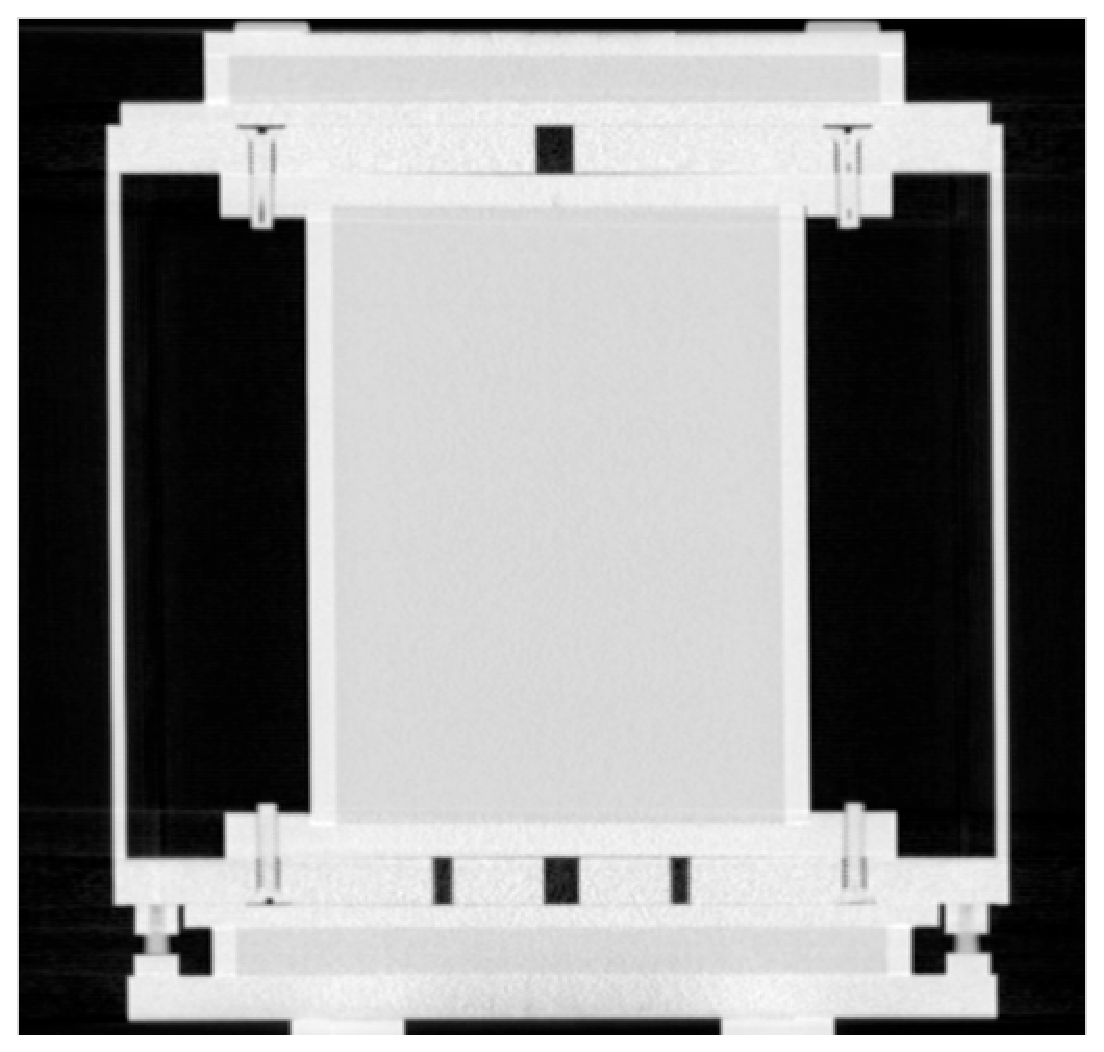
\includegraphics[width=2.75in]{data_extraction/images/targets/ct_coronal_mid_slice.eps}}}
    \centerline{\emph{(a) Coronal view, center slice}}
  \end{minipage}\medskip
  \begin{minipage}[t]{2.75in}
    \centering
    \centerline{\mbox{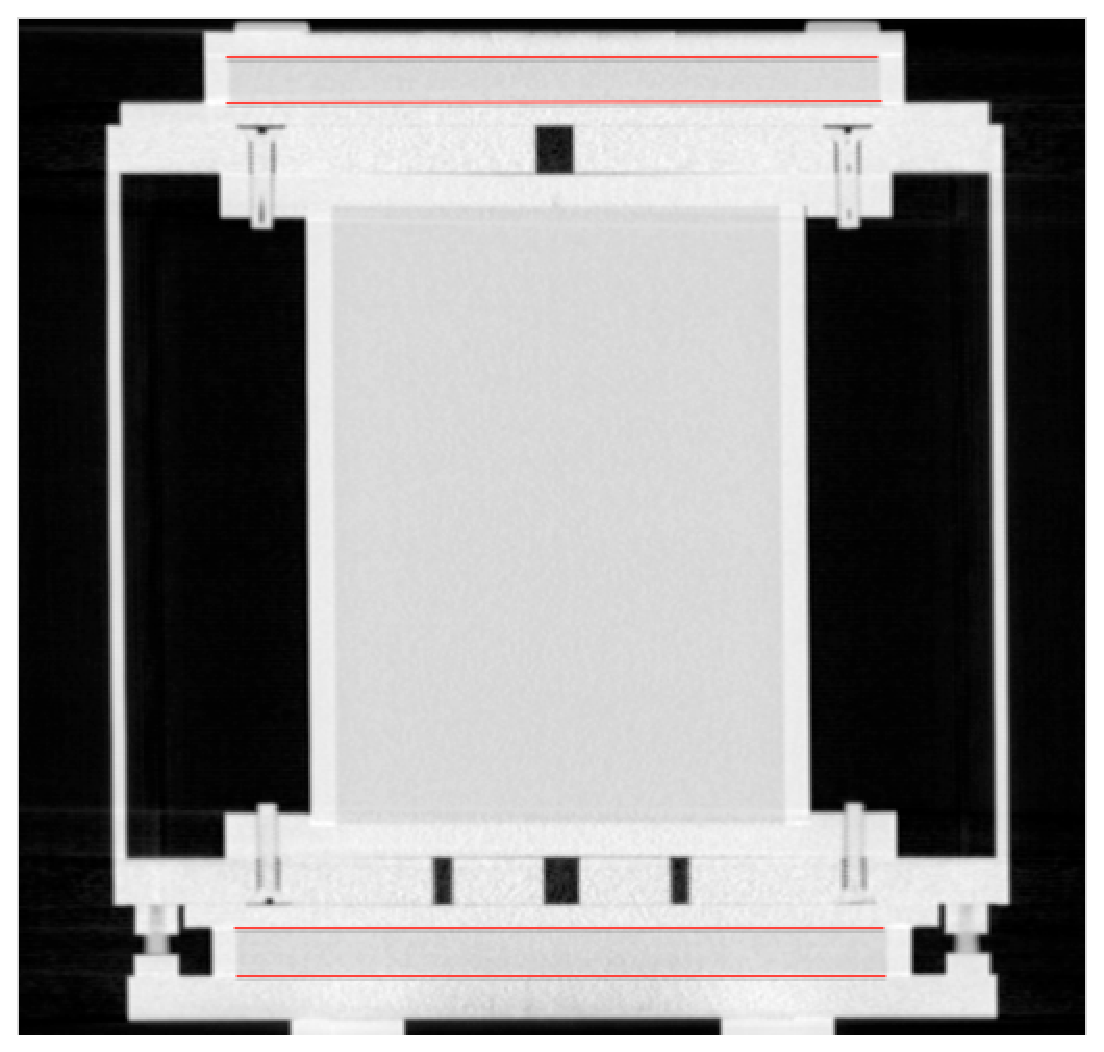
\includegraphics[width=2.75in]{data_extraction/images/targets/ct_coronal_mid_slice_marked_surface.eps}}}
    \centerline{\emph{(b) Marked target surfaces}}
  \end{minipage}
\end{figure}

\subsection{Canny Edges}
\begin{figure}[htb]
  \begin{minipage}[t]{2.75in}
    \centering
    \centerline{\mbox{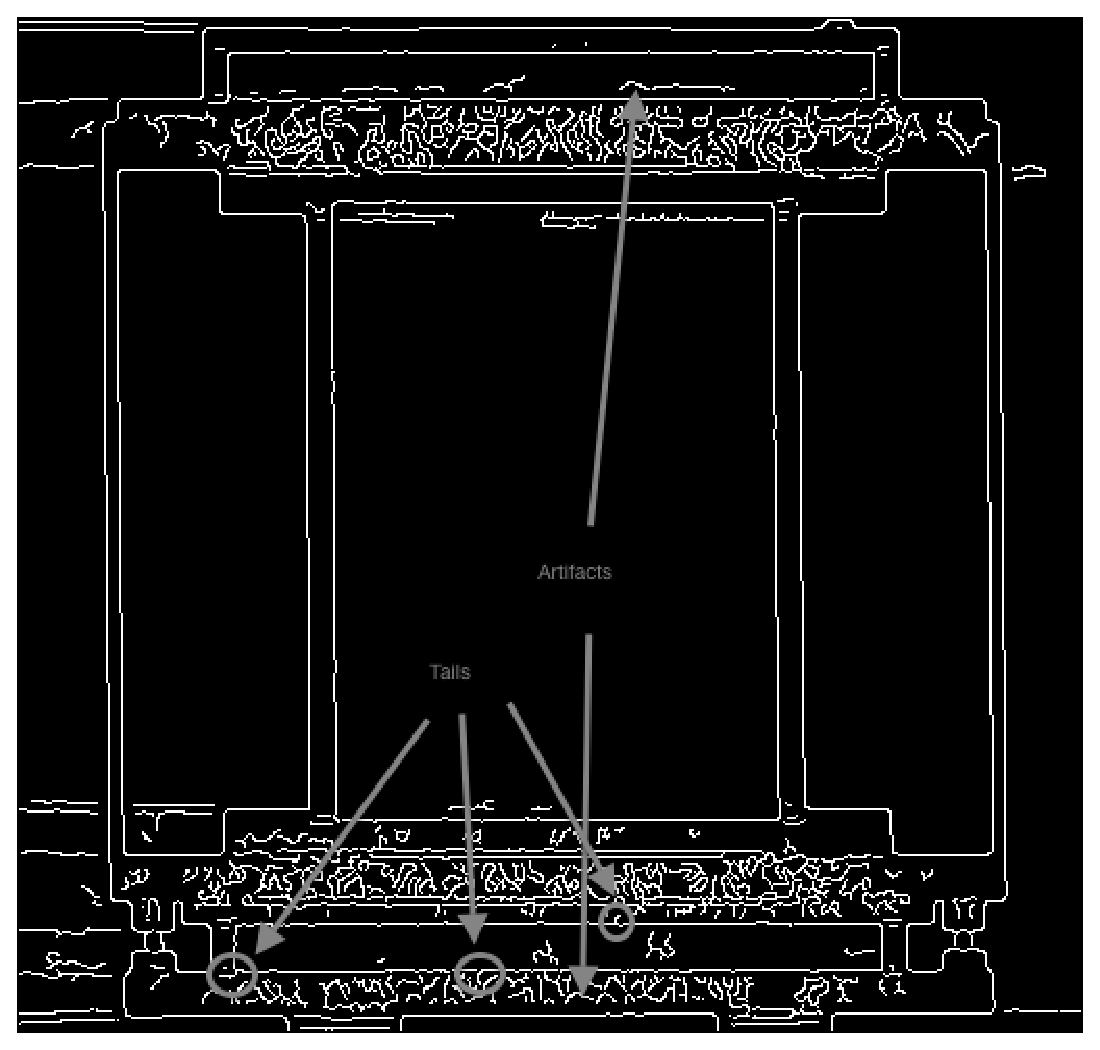
\includegraphics[width=2.75in]{data_extraction/images/canny/cases/Canny_issue_artifacts.eps}}}
    \centerline{\emph{(a) Artifacts in canny edges}}
  \end{minipage}\medskip
  \begin{minipage}[t]{2.75in}
    \centering
    \centerline{\mbox{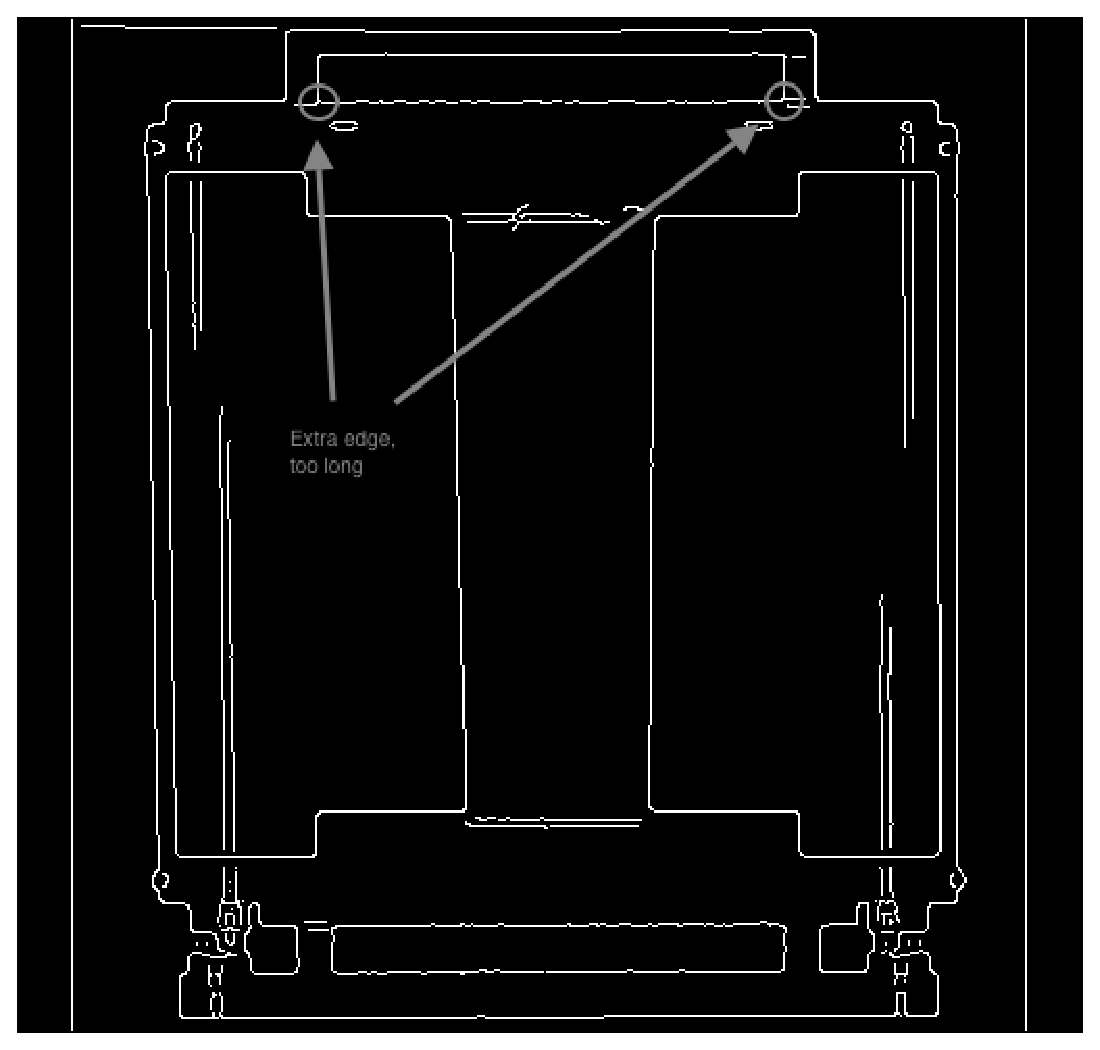
\includegraphics[width=2.75in]{data_extraction/images/canny/cases/Canny_issue_relatively_better.eps}}}
    \centerline{\emph{(b) Relatively better result}}
  \end{minipage}
  \begin{minipage}[t]{2.75in}
    \centering
    \centerline{\mbox{
\includegraphics[width=2.75in]{data_extraction/images/canny/cases/Canny_issue_high_threshold.eps}}}
    \centerline{\emph{(c) High threshold result}}
  \end{minipage}\medskip
  \begin{minipage}[t]{2.75in}
    \centering
    \centerline{\mbox{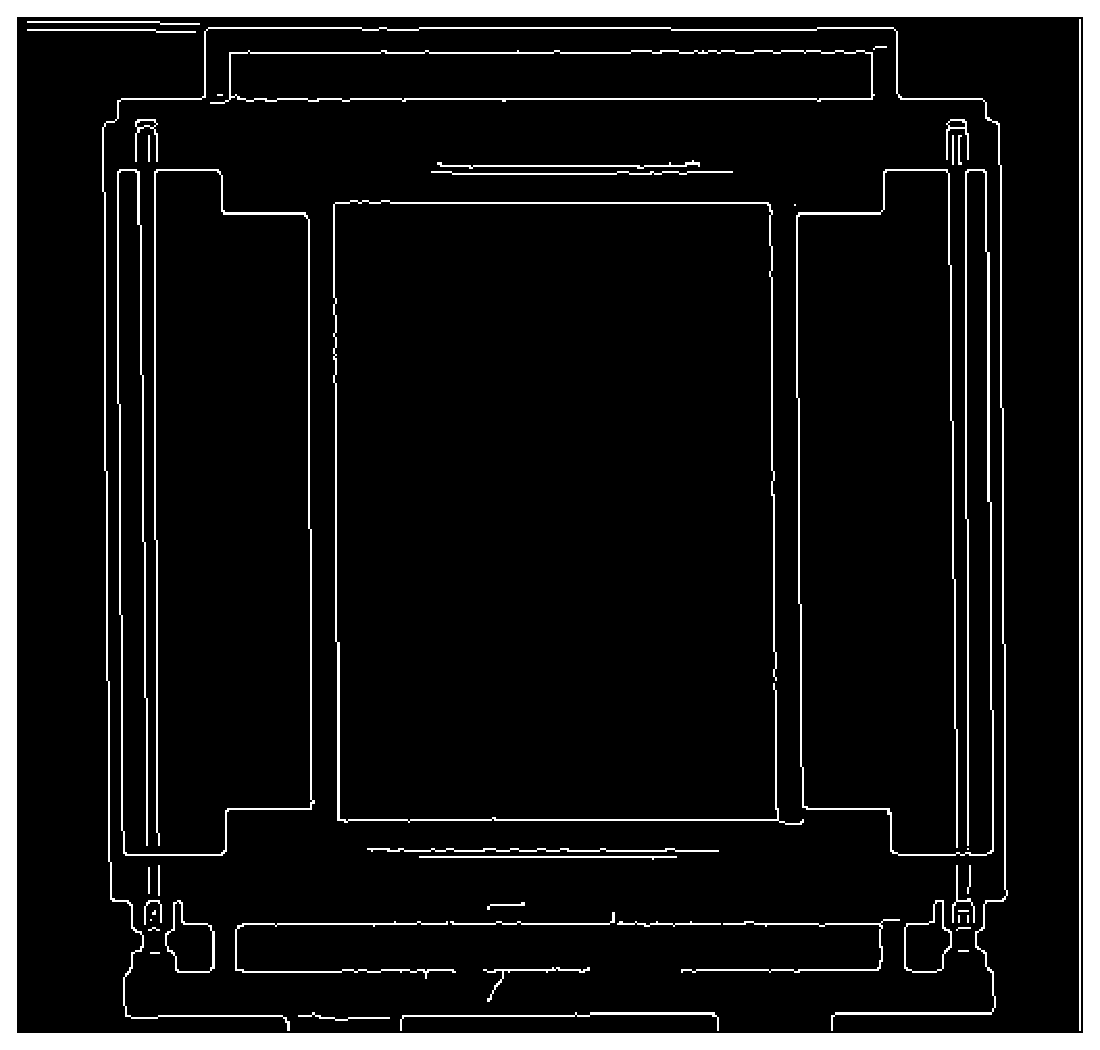
\includegraphics[width=2.75in]{data_extraction/images/canny/cases/Canny_issue_missing_edges.eps}}}
    \centerline{\emph{(d) Incomplete edges}}
  \end{minipage}

\end{figure}



\subsection{Surface Location}

\subsection{Canny On Local Region}

\subsection{Removing Extra Edges}

\subsection{Creating Surfaces}

\subsection{Estimating Surfaces Distances}

